\documentclass[a4paper,14pt]{extarticle}

\usepackage[utf8x]{inputenc}
\usepackage[T1,T2A]{fontenc}
\usepackage[russian]{babel}
\usepackage{hyperref}
\usepackage{indentfirst}
\usepackage{here}
\usepackage{array}
\usepackage{graphicx}
\usepackage{caption}
\usepackage{subcaption}
\usepackage{chngcntr}
\usepackage{amsmath}
\usepackage{amssymb}
\usepackage{pgfplots}
\usepackage{pgfplotstable}
\usepackage[left=2cm,right=2cm,top=2cm,bottom=2cm,bindingoffset=0cm]{geometry}
\usepackage{multicol}

\renewcommand{\le}{\ensuremath{\leqslant}}
\renewcommand{\leq}{\ensuremath{\leqslant}}
\renewcommand{\ge}{\ensuremath{\geqslant}}
\renewcommand{\geq}{\ensuremath{\geqslant}}
\renewcommand{\epsilon}{\ensuremath{\varepsilon}}
\renewcommand{\phi}{\ensuremath{\varphi}}

\counterwithin{figure}{section}
\counterwithin{equation}{section}
\counterwithin{table}{section}
\newcommand{\sign}[1][5cm]{\makebox[#1]{\hrulefill}} % Поля подписи и даты
\graphicspath{{pics/}} % Путь до папки с картинками
\captionsetup{justification=centering,margin=1cm}
\def\arraystretch{1.3}

\begin{document}	% начало документа

\begin{titlepage}
\begin{center}
	\textbf{Санкт-Петербургский Политехнический Университет \\Петра Великого}\\[0.3cm]
	\small Институт компьютерных наук и технологий \\[0.3cm]
	\small Кафедра компьютерных систем и программных технологий\\[4cm]
	
	\textbf{ОТЧЕТ}\\ \textbf{о лабораторной работе}\\[0.5cm]
	\textbf{<<Исследование частотных характеристик пассивных RC-цепей>>}\\[0.1cm]
	\textbf{Электротехника и Электроника}\\[10.5cm]
\end{center}

\begin{flushright}
	\begin{minipage}{0.60\textwidth}
		\begin{flushleft}
			\small \textbf{Работу выполнили студенты}\\[3mm]
			\small группа 23501/4 \hspace*{17mm} Дьячков В.В.\\[3mm]
			\small группа 23501/4 \hspace*{17mm} Ламтев А.Ю.\\[5mm]
			
			\small \textbf{Преподаватель}\\[5mm]
		 	\small \sign[3.5cm] \hspace*{8mm} к.т.н., доц. Кочетков Ю.Д.\\[0.5cm]
		\end{flushleft}
	\end{minipage}
\end{flushright}

\vfill

\begin{center}
	\small Санкт-Петербург\\
	\small \the\year
\end{center}
\end{titlepage}


\section{Цель работы}
Исследовать частотные свойства простейших пассивных RC­-цепей и познакомиться с правилами построения частотных характеристик.


\section{Чертеж схемы исследуемого устройства}
\begin{figure}[h]
\centering
\begin{subfigure}[b]{0.34\textwidth}
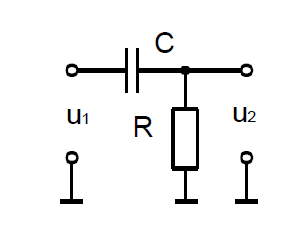
\includegraphics[scale=0.4]{a_scheme.png}
\caption{Дифференцирующая\\ цепь}\label{figure:2.1:a}
\end{subfigure}
\begin{subfigure}[b]{0.3\textwidth}
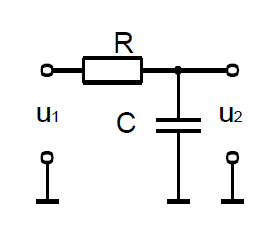
\includegraphics[scale=0.4]{b_scheme.png}
\caption{Интегрирующая\\ цепь}\label{figure:2.1:b}
\end{subfigure}
\begin{subfigure}[b]{0.3\textwidth}
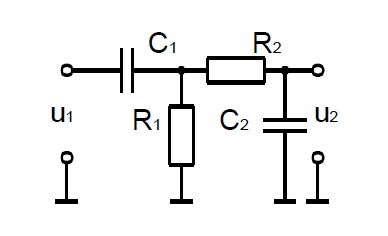
\includegraphics[scale=0.4]{v_scheme.png}
\caption{Дифференцирующая и интегрирующая цепь}\label{figure:2.1:c}
\end{subfigure}
\caption{}\label{figure:2.1}
\end{figure}
На рисунке \ref{figure:2.1:a} изображена дифференцирующая RC-цепь, на (\ref{figure:2.1:b}) - интегрирующая RC-цепь, и на  (\ref{figure:2.1:c}) - последоватльное соединение дифференцирующей и интегрирующей RC-­цепей.


\section{Исходные данные}
Исходные значения были подобраны следующим образом:
\begin{center}
\begin{tabular}{|c|c|}
\hline 
$R$ & 15 кОм \\ 
\hline 
$C$ & 5 нФ \\ 
\hline 
\end{tabular}  
\end{center}


\section{Расчет элементов и параметров схемы}
Частота перегиба расчитывается следующим образом:
\begin{equation}
\omega_0 = \frac{1}{RC} = \frac{1}{15 \cdot 10^3 \cdot 5 \cdot 10^{-9}} \simeq 1.334 \cdot 10^4 \hspace*{2mm}
\end{equation}
Отсюда: 
\begin{equation}
f_0 = \frac{\omega_0}{2 \pi} = \frac{1.34}{2\cdot1.341} \simeq 2122.065   
\end{equation}
Теоретическая ЛАЧХ для дифференцирующей RC-цепи строится по
формуле
\begin{equation}
L_u(\omega) = 20lg \omega RC - 10lg(1+(\omega RC)^2),
\end{equation}
для построения ЛАЧХ интегрирующей RC-цепи используется выражение
\begin{equation}
L_u(\omega) = - 10lg(1+(\omega RC)^2),
\end{equation}
а ЛАЧХ соеденных последовательно дифференцирующей и интегриущей цепей рассчитывается по формуле
\begin{equation}
L_u(\omega) = 20lg \omega RC - 10lg(1+7(\omega RC)^2 + (\omega RC)^4).
\end{equation}


\section{Теоретические зависимости}

\begin{center}
\begin{table}[h]
\caption{Значения для построения теоретических ЛАЧХ}
\pgfplotstabletypeset[col sep=comma,
    columns={f,w,L1,L2,L3},
    column type/.add={|c|}{},
    columns/f/.style={fixed, column name={$f,$ Гц}},
    columns/w/.style={fixed, precision=3, column name={$\omega = 2 \pi f$ }},
    columns/L1/.style={fixed, precision=3, column name={$L_{\text{диф.}}$, дБ}},
    columns/L2/.style={fixed, precision=3, column name={$L_{\text{инт.}}$, дБ}},
    columns/L3/.style={fixed, precision=3, column name={$L_{\text{соед.}}$, дБ}},
    every nth row={1}{before row=\hline},
    every head row/.style = {before row=\hline, after row=\hline},
    every last row/.style = {after row=\hline}
   ]{adata.csv}
\end{table}
\end{center}
    
\subsection{Экспериментально снятые зависиости}
В таблицах \ref{t:e1}, \ref{t:e2} и \ref{t:e3} приведены значения входного напряжения, выходного напряжения, коэффициента передачи и коэффициента передачи, выраженного в децибелах, дифференцирующей RC-цепи, для интегрирующей RC-цепи и соединенных последовательно дифференцирующей и интегрирующей RC-цепей соответсвенно. 

На рисунках \ref{t:e1}, \ref{t:e2} и \ref{t:e3} приведены теоритические ЛАЧХ, экспериментальные ЛАЧХ и аппроксимирующие прямые для всех цепей.

Для каждой из полученных зависимостей было выполнено интерполирование в области частоты перегиба $f_0 = 2122.065$ Гц: был построен интерполяционный полином по трем точкам, значение частоты которых наиболее близко к частоте пергиба, а именно $f_1 = 1024$, $f_2 = 2048$, $f_3 = 4096$.  

Интерполяционный полином ЛАЧХ дифференцирующей RC-цепи в области частоты перегибы имеет вид:
\begin{equation}
L_u(f) = -13.393 + (6.81 \cdot 10^{-3})f + (-9.474 \cdot 10^{-7})f^2. 
\end{equation}
Для ЛАЧХ интергрирующей RC-цепи аналогичный интерполяционный полином представляет собой выражение
\begin{equation}
L_u(f) = -0.744 + (2.013 \cdot 10^{-3})f + (-1.303 \cdot 10^{-8})f^2.
\end{equation}
Интерполяционны полином ЛАЧХ соединенных последовательно интергрирующей и дифференцирующей RC-цепей выглядит следующим образом:
\begin{equation}
L_u(f) = -12.667 + (2.186 \cdot 10^{-3})f + (-4.242 \cdot 10^{-7})f^2.
\end{equation}

Предельная допустимая относительная погрешность для дифференцирующей и интегрирующей цепей составляет
\begin{equation}
\delta f_0 = \sqrt{(\delta R)^2 + (\delta C)^2} = \sqrt{0.01 + 0.01} = 0.1414
\end{equation} 

Для дифференцирующей и интегрирующей цепи:
\begin{equation}
\delta f_0 = \sqrt{2 \cdot (\delta R)^2 + 2 \cdot (\delta C)^2} = \sqrt{0.01 + 0.01} = 0.2
\end{equation} 

На основе полученных выражений и с учетом погрешности были рассчитаны значения ЛАЧХ в точке перегиба для всех цепей:\\
$L_u(f_0)_\text{дифф} = -3.427 \pm 0.485$ (дБ)\\ 
$L_u(f_0)_\text{инт} = -3.350 \pm 0.473$ (дБ)\\
$L_u(f_0)_\text{дифф-инт} = -9.546 \pm 1.350$ (дБ)\\
 
\begin{table}[!h]
\caption{Коэффициент передачи дифференциующей RC-цепи.}
\pgfplotstabletypeset[col sep=comma,
    columns={f,Ui,Uo,K,L},
    column type/.add={|c|}{},
    columns/f/.style={fixed, column name={$f$, Гц}},
    columns/Ui/.style={fixed, precision=3, column name={$U_{\text{вх}}$, В}},
    columns/Uo/.style={fixed, precision=3, column name={$U_{\text{вых}}$, В}},
    columns/K/.style={fixed, precision=3, column name={$K$, В}},
    columns/L/.style={fixed, precision=3, column name={$-20 \cdot lg(K)$, дБ}},
    every nth row={1}{before row=\hline},
    every head row/.style = {before row=\hline, after row=\hline, fixed},
    every last row/.style = {after row=\hline, fixed}
   ]{e1data.csv}
\label{t:e1}
\end{table}

\begin{figure}[h]
\begin{tikzpicture}
\begin{axis}[
	legend pos=north west,
	ylabel near ticks,
	xlabel near ticks,
    xmode=log,
    width=0.85\textwidth,
    log basis x={2},
	xlabel={$f$, Гц},
	ylabel={$L_u$, Дб},
	%ylabel style={rotate=-90},
	xtick={0, 32, 128, 512, 2048, 8192, 32768, 131072},
	xticklabel style={/pgf/number format/.cd,fixed,precision=2}
]
\addplot table [x=f, y=L1, col sep=comma] {adata.csv};
\addplot table [x=f, y=L, col sep=comma] {e1data.csv};
\addplot +[mark=none, dashed, black, samples=2] coordinates {(2048,0) (131072,0)};
\addplot +[mark=none, dashed, black, domain=32:2200] {-(log2(x)*(-6)+66.3)};
\legend{Teор. ЛАЧХ, Эксп. ЛАЧХ}
\end{axis}
\end{tikzpicture} \hfill
\label{f:e1}
\caption{Теоретическая и экспериментальная ЛАЧХ дифференцирующей RC-цепи}
\end{figure}


\begin{table}[!h]
\caption{Коэффициент передачи интегрирующей RC-цепи.}
\pgfplotstabletypeset[col sep=comma,
    columns={f,Ui,Uo,K,L},
    column type/.add={|c|}{},
    columns/f/.style={fixed, column name={$f$, Гц}},
    columns/Ui/.style={fixed, precision=3, column name={$U_{\text{вх}}$, В}},
    columns/Uo/.style={fixed, precision=3, column name={$U_{\text{вых}}$, В}},
    columns/K/.style={fixed, precision=3, column name={$K$, В}},
    columns/L/.style={fixed, precision=3, column name={$-20 \cdot lg(K)$, дБ}},
    every nth row={1}{before row=\hline},
    every head row/.style = {before row=\hline, after row=\hline, fixed},
    every last row/.style = {after row=\hline, fixed}
   ]{e2data.csv}
\label{t:e2}
\end{table}

\begin{figure}[h]
\label{f:e2}
\begin{tikzpicture}
\begin{axis}[
	ylabel near ticks,
	xlabel near ticks,
	legend pos=north east,
    xmode=log,
    width=0.85\textwidth,
    log basis x={2},
	xlabel={$f$, Гц},
	ylabel={$L_u$, Дб},
	%ylabel style={rotate=-90},
	xtick={0, 32, 128, 512, 2048, 8192, 32768, 131072},
	xticklabel style={/pgf/number format/.cd,fixed,precision=2}
]
\addplot table [x=f, y=L2, col sep=comma] {adata.csv};
\addplot table [x=f, y=L, col sep=comma] {e2data.csv};
\addplot +[mark=none, dashed, black, samples=2] coordinates {(32,0) (2300,0)};
\addplot +[mark=none, dashed, black, domain=2048:131072] {log2(x)*(-6)+66.3};
\legend{Teор. ЛАЧХ, Эксп. ЛАЧХ}
\end{axis}
\end{tikzpicture} \hfill
\caption{Теоретическая и экспериментальная ЛАЧХ интегрирующей RC-цепи}
\end{figure}


\begin{table}[!h]
\caption{Коэффициент передачи дифференциующей и интегрирующей  RC-цепей, соединенных последовательно.}
\pgfplotstabletypeset[col sep=comma,
    columns={f,Ui,Uo,K,L},
    column type/.add={|c|}{},
    columns/f/.style={fixed, column name={$f$, Гц}},
    columns/Ui/.style={fixed, precision=3, column name={$U_{\text{вх}}$, В}},
    columns/Uo/.style={fixed, precision=3, column name={$U_{\text{вых}}$, В}},
    columns/K/.style={fixed, precision=3, column name={$K$, В}},
    columns/L/.style={fixed, precision=3, column name={$-20 \cdot lg(K)$, дБ}},
    every nth row={1}{before row=\hline},
    every head row/.style = {before row=\hline, after row=\hline, fixed},
    every last row/.style = {after row=\hline, fixed}
   ]{e3data.csv}
\label{t:e3}
\end{table}


\begin{figure}[h]
\label{f:e3}
\begin{tikzpicture}
\begin{axis}[
	ylabel near ticks,
	xlabel near ticks,
	legend pos=north east,
    xmode=log,
    width=0.85\textwidth,
    log basis x={2},
	xlabel={$f$, Гц},
	ylabel={$L_u$, Дб},
	%ylabel style={rotate=-90},
	xtick={0, 32, 128, 512, 2048, 8192, 32768, 131072},
	xticklabel style={/pgf/number format/.cd,fixed,precision=2}
]
\addplot table [x=f, y=L3, col sep=comma] {adata.csv};
\addplot table [x=f, y=L, col sep=comma] {e3data.csv};
\addplot +[mark=none, dashed, black, domain=2000:131072] {log2(x)*(-6)+66.3};
\addplot +[mark=none, dashed, black, domain=32:2280] {-(log2(x)*(-6)+66.3)};
\legend{Teор. ЛАЧХ, Эксп. ЛАЧХ}
\end{axis}
\end{tikzpicture} \hfill
\caption{Теоретическая и экспериментальная ЛАЧХ соединенных последовательно интегрирующей и дифференцирующей RC-цепей}
\end{figure}
\end{document}
